\chapter{Lezione 5 - Architettura di Enterprise Resource Planning System}

Benvenuti a questa nuova lezione sull'architettura di un Enterprise Resource Planning System.
Tratteremo gli aspetti della comunicazione.
Gli argomenti trattati saranno quindi l'architettura orientata ai servizi SOA e la gestione dei servizi web.

Argomenti trattati:

\FloatBarrier
\begin{figure}[H]
  \centering
  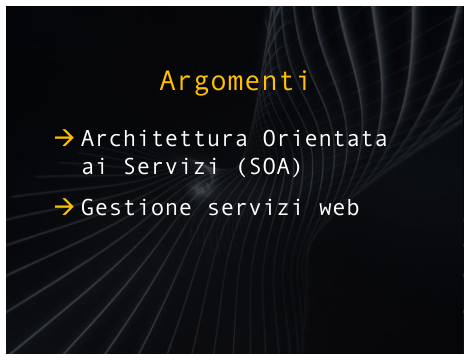
\includegraphics[width=0.50\textwidth,
                    trim=40 100 40 60, % L B R T
                    clip]
                    {images/Lez05_p01_fig_02}
  % \caption{Sommario}
  % \label{fig:Lez15_p06_fig_02}
\end{figure}
\FloatBarrier
\noindent


Cominciamo con l'architettura orientata ai servizi.

Innanzitutto, l'Oasis ha fornito la definizione di questo tipo di architettura.
L'Oasis è acronimo per Organization for the Advancement of Structured Information Standards.
Organizzazione per l'avanzamento degli standard per le informazioni strutturate.

E' un consorzio no-profit con sede negli Stati Uniti e composta da più di 5.000 partecipanti che rappresentano 600 organizzazioni in più di 65 paesi in giro per il mondo.
Si occupa dello sviluppo, la convergenza e l'adozione, quindi la promozione, di standard aperti per l'organizzazione di web services, che vedremo nel corso di questa lezione cosa sono e come vengono utilizzati.
Questa organizzazione, l'Oasis, ha proposto una definizione, ora divenuta, di riferimento per la SOA, per la Simple Object Architecture.

\FloatBarrier
\begin{figure}[H]
  \centering
  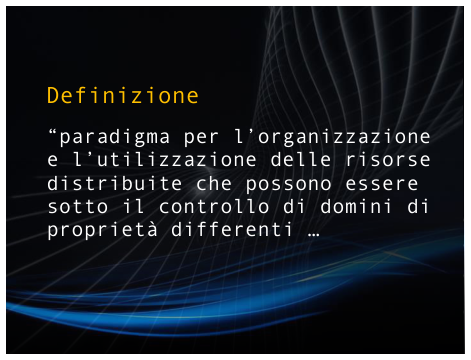
\includegraphics[width=0.50\textwidth,
                    trim=20 100 20 60, % L B R T
                    clip]
                    {images/Lez05_p01_fig_04}
  % \caption{Sommario}
  % \label{fig:Lez15_p06_fig_02}
\end{figure}
\FloatBarrier
\noindent


E' un paradigma per l'organizzazione e l'utilizzazione delle risorse distribuite che possono essere sotto il controllo di domini di proprietà differenti.

\FloatBarrier
\begin{figure}[H]
  \centering
  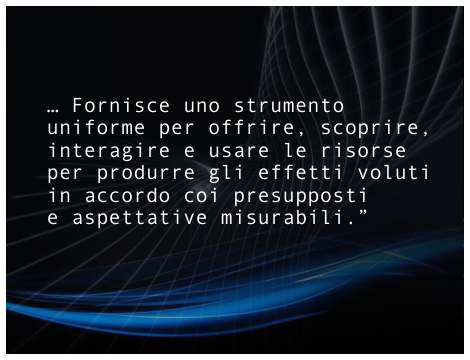
\includegraphics[width=0.50\textwidth,
                    trim=20 100 20 60, % L B R T
                    clip]
                    {images/Lez05_p01_fig_05}
  % \caption{Sommario}
  % \label{fig:Lez15_p06_fig_02}
\end{figure}
\FloatBarrier
\noindent

Fornisce uno strumento uniforme per offrire, scoprire, interagire e usare le risorse per produrre gli effetti voluti in accordo con i presupposti e aspettative misurabili.
Vorrei spendere alcune parole di interpretazione di questa definizione.
Innanzitutto è un paradigma.
Quindi siamo a livello di specifiche, siamo a livello di modello, siamo a livello di una definizione che è utilizzata come riferimento per progettare servizi complessi, progettare applicazioni basate sui servizi complessi.

Le risorse possono essere distribuite.
Risorse distribuite vuol dire che stiamo parlando di architetture che non sono necessariamente installate su un singolo host, su una singola macchina o che non sono locali.
Sono architetture che compongono servizi che possono essere gestiti da macchine remote e sotto domini differenti, quindi sotto il controllo, sotto il governo, differenti.
Questo complica enormemente l'implementazione e la progettazione, quindi, di queste architetture.

\FloatBarrier
\begin{figure}[H]
  \centering
  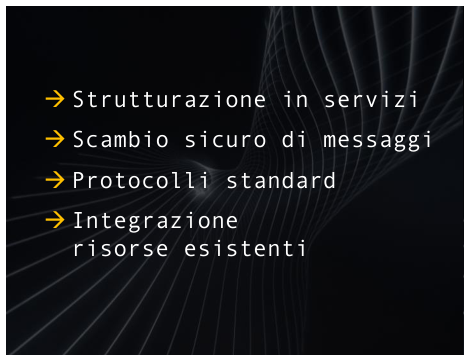
\includegraphics[width=0.50\textwidth,
                    trim=20 80 20 60, % L B R T
                    clip]
                    {images/Lez05_p02_fig_01}
  % \caption{Sommario}
  % \label{fig:Lez15_p06_fig_02}
\end{figure}
\FloatBarrier
\noindent

Le tecnologie basate su questo paradigma permettono innanzitutto la strutturazione in servizi, o sarebbe più corretto dire implicano la strutturazione in servizi.
Questo tipo di architettura implica, richiede, una prospettiva in cui le necessità dell'utente siano soddisfatte da un sistema che permetta l'erogazione di servizi, permetta l'erogazione di attività automatizzate che possano essere configurate o chiamate servizi.

Questa architettura è basata sullo scambio sicuro di messaggi tra i vari elementi, tra i vari moduli, che implementano i singoli servizi da comporre per erogare il servizio che soddisferrà o cercherà di soddisfare le richieste dell'utente.

Questa architettura è basata su protocolli standard, protocolli per l'interoperabilità, protocolli per lo scambio dei messaggi, ma anche protocolli per la codifica, quindi per il confezionamento di questi messaggi, che sono usati per lo scambio di messaggi e per la comunicazione, quindi per lo scambio di informazioni ancillari per il funzionamento del sistema complesso.

Inoltre, questa architettura è basata sull'integrazione di sistemi esistenti, quindi si punta a una architettura, a un sistema che possa essere esteso a livello di principio di programmazione, siamo di principio ideativo, di principio di paradigma, una struttura di base che possa essere estesa con ulteriori servizi, con ulteriori applicazioni proposte, sviluppate e fornite da altri domini, da altri fornitori, gestiti da altri calcolatori.

\FloatBarrier
\begin{figure}[H]
  \centering
  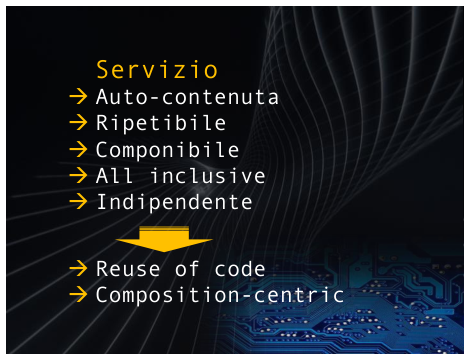
\includegraphics[width=0.50\textwidth,
                    trim=20 20 20 40, % L B R T
                    clip]
                    {images/Lez05_p02_fig_02}
  % \caption{Sommario}
  % \label{fig:Lez15_p06_fig_02}
\end{figure}
\FloatBarrier
\noindent


Ma che cos'è un servizio?
Un servizio è un'applicazione, o meglio è l'attività erogata da un'applicazione autocontenuta, cioè l'elemento di software, l'applicativo che svolge il singolo servizio, deve contenere tutti gli elementi di calcolo attivi, tutte le operazioni e tutte le informazioni, i dati, che servono per realizzare quello specifico minimale servizio, minimale attività.

Ogni servizio deve essere ripetibile.
Ogni servizio deve essere ripetibile quante volte è necessario e su richiesta di qualsivoglia altro servizio che invi una richiesta attraverso un messaggio ben formato secondo il protocollo richiesto dalla Service Oriented Architecture.

I servizi sono componibili, perché sono i mattoncini o si parla di granularità, sono gli elementi basilari componibili per costruire un servizio più complesso da fornire all'utente.

Ma è rilevante che ogni servizio, ogni modulo realizzativo di un servizio sia all inclusive.
Come abbiamo detto, gli elementi implementati devono essere autonomi per quanto riguarda le attività necessarie e i dati necessari a svolgere queste attività.

Questi moduli devono essere indipendenti.
Indipendenti significa che questi moduli non dipendono funzionalmente dagli altri moduli, ma gli altri moduli devono essere a conoscenza dei moduli utili allo svolgimento complessivo del servizio complesso e con loro possano interagire per richiedere la loro attivazione attraverso scambio di messaggi.

Questo permette il riuso dei sorgenti per comporre servizi più complessi e il punto focale di questo paradigma è la componibilità, quindi il riuso dei componenti per comporre nuovi e più complessi servizi.

\FloatBarrier
\begin{figure}[H]
  \centering
  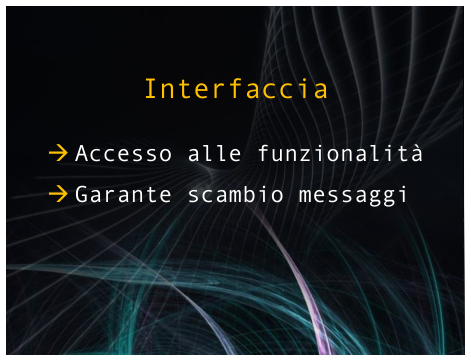
\includegraphics[width=0.50\textwidth,
                    trim=20 120 20 60, % L B R T
                    clip]
                    {images/Lez05_p02_fig_03}
  % \caption{Sommario}
  % \label{fig:Lez15_p06_fig_02}
\end{figure}
\FloatBarrier
\noindent

Un elemento importante per l'implementazione dei servizi è l'interfaccia.
L'interfaccia è la descrizione delle modalità di accesso alle funzionalità offerte da quel modulo.
L'interfaccia offre anche una garanzia sullo scambio dei messaggi, quindi doppia funzionalità, descrizione, presentazione, quindi in qualche modo il metadato, presentazione del tipo di attività che può essere svolta, dal tipo di servizio elementare che può essere erogato e dall'altra parte correzione, rifiuto o esecuzione dei messaggi di richiesta che vengono ricevuti dall'interfaccia o invio per attivazione o ricerca di ulteriori servizi.

\FloatBarrier
\begin{figure}[H]
  \centering
  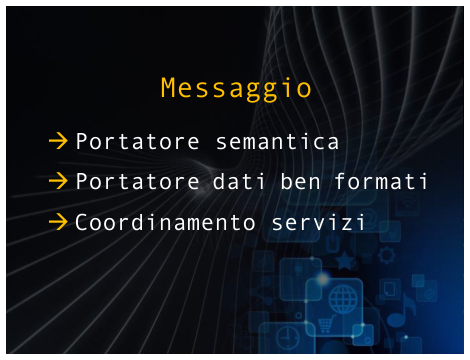
\includegraphics[width=0.50\textwidth,
                    trim=20 120 20 60, % L B R T
                    clip]
                    {images/Lez05_p02_fig_04}
  % \caption{Sommario}
  % \label{fig:Lez15_p06_fig_02}
\end{figure}
\FloatBarrier
\noindent

Un messaggio, un messaggio previsto dall'architettura Service Oriented è portatore di semantica.

Portatore di semantica vuol dire che di base vengono utilizzati per la richiesta, quindi per la collezione dei vari elementi attivi che costituiscano il complesso sistema e il loro coordinamento.

Un messaggio è un portatore di dati ben formati, quindi il messaggio porta un significato, porta la descrizione di un'attività, ma deve essere descritto secondo un preciso protocollo che vedremo.

I messaggi sono definiti con l'obiettivo di coordinare questi servizi, quindi sono messaggi che hanno una loro costituzione ben specifica e particolare per il coordinamento delle attività service oriented.

\FloatBarrier
\begin{figure}[H]
  \centering
  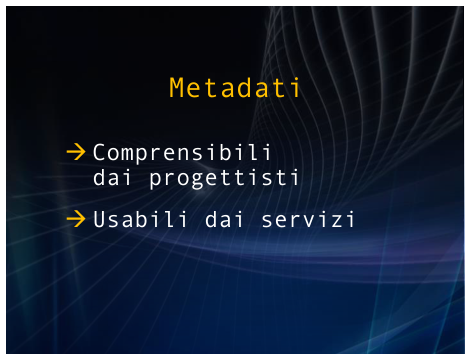
\includegraphics[width=0.50\textwidth,
                    trim=20 120 20 60, % L B R T
                    clip]
                    {images/Lez05_p02_fig_05}
  % \caption{Sommario}
  % \label{fig:Lez15_p06_fig_02}
\end{figure}
\FloatBarrier
\noindent

Alla base dei servizi ci sono i metadati.
I metadati sono comprensibili dai progettisti e usabili dai servizi.
Che cosa intendiamo?
I metadati sono descrizioni delle informazioni che vengono utilizzate per costituire i servizi e dagli applicativi, dagli elementi software, che verranno utilizzati per realizzare questi servizi.
Allora i metadati dovranno avere una forma e una descrizione che sia utilizzabile da chi progetta i sistemi complessi, quindi degli uomini, ma siano anche nella stessa forma utilizzabili, comprensibili dalle applicazioni che li utilizzeranno.

Consideriamo questo primo argomento concluso e quindi vi propongo uno spunto di riflessione.
Provate a descrivere un esempio di servizio e una modalità di riuso che sia riferito al vostro ambito di lavoro o all'ambito formativo universitario che frequentate.

\section{Gestione servizi web}

\FloatBarrier
\begin{figure}[H]
  \centering
  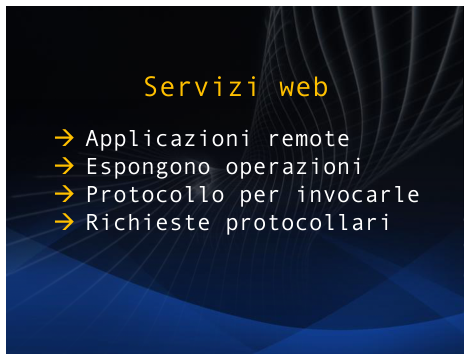
\includegraphics[width=0.50\textwidth,
                    trim=20 120 20 60, % L B R T
                    clip]
                    {images/Lez05_p03_fig_02}
  % \caption{Sommario}
  % \label{fig:Lez15_p06_fig_02}
\end{figure}
\FloatBarrier
\noindent

Vediamo ora la gestione dei servizi web.
Cos'è un servizio web?
Innanzitutto è un'applicazione remota.
Ricordiamo che la definizione dell'Oasis sulla architettura orientata agli oggetti era paradigma per applicazioni eventualmente sotto i sottodomini diversi.
Le applicazioni possono essere remote.
Il servizio che la nostra organizzazione eroga per costituire l'enterprise resource planning che utilizza non è necessariamente erogato da una macchina, da un host locale. Può essere un host da qualsiasi parte.
Si parla quindi di servizi alocalizzati.

Sarà importante però che ogni servizio esponga le proprie operazioni, cioè presenti descriva in qualche modo, quindi secondo un protocollo che vedremo, il proprio funzionamento, le proprie modalità di accesso e il tipo di attività che è in grado di svolgere.

Vediamo che è richiesto un protocollo per invocare sia un protocollo per ricercare queste applicazioni remote adatte al nostro scopo, sia per richiedere il servizio di quell'applicazione che abbiamo recuperato.

Il quarto punto che riguarda i servizi web sono le richieste protocollari.
Un servizio web è cercato e richiesto secondo specifici protocolli.

\FloatBarrier
\begin{figure}[H]
  \centering
  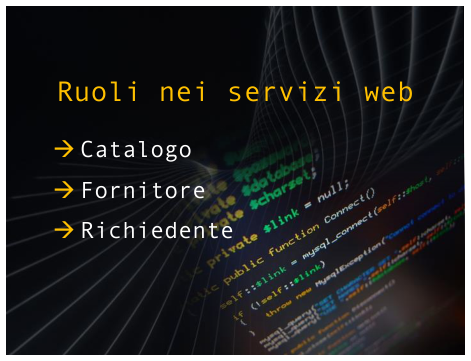
\includegraphics[width=0.50\textwidth,
                    trim=20 100 20 60, % L B R T
                    clip]
                    {images/Lez05_p03_fig_03}
  % \caption{Sommario}
  % \label{fig:Lez15_p06_fig_02}
\end{figure}
\FloatBarrier
\noindent

Vi sono alcuni ruoli basilari per attivare o partecipare, sviluppare, entrare nel meccanismo, sviluppare un'applicazione che eroghi un servizio basato sui servizi web, sui web services.

Dobbiamo considerare il primo elemento in catalogo.
Cos'è il catalogo?
Il catalogo è un archivio che contiene i servizi pubblici, i servizi che possono essere utilizzati, ricercati.
Allora i servizi saranno descritti secondo un opportuno protocollo, WSDL, Web Service Description Language, o meglio il funzionamento dei servizi, il funzionamento di ogni web service sarà descritto secondo questo linguaggio, utilizzando le specifiche di questo linguaggio.

Il fornitore è colui che avendo realizzato un servizio di cui un modulo, che eroga un servizio di cui riconosce la pubblica utilità, inserisce con l'opportuna descrizione il nuovo servizio nel catalogo, nell'archivio offerto a pubblico dominio.

Il richiedente è l'utente che cerca uno specifico servizio.
Il richiedente può essere riferita come la persona che in quel momento ha bisogno di un nuovo servizio per svolgere una sua attività, per soddisfare una propria necessità informativa o computazionale, o può essere un'applicazione che utilizzando l'opportuno protocollo richiede al catalogo la disponibilità di servizi che svolgano opportune attività.

\FloatBarrier
\begin{figure}[H]
  \centering
  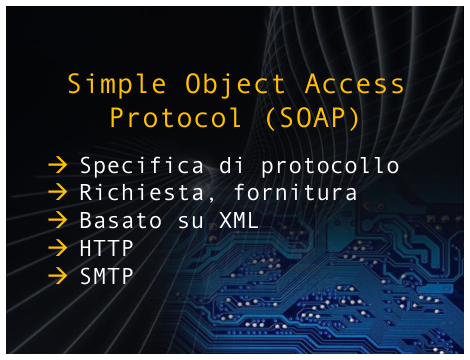
\includegraphics[width=0.50\textwidth,
                    trim=20 100 20 60, % L B R T
                    clip]
                    {images/Lez05_p03_fig_04}
  % \caption{Sommario}
  % \label{fig:Lez15_p06_fig_02}
\end{figure}
\FloatBarrier
\noindent

Un protocollo di comunicazione per la ricerca di servizi web è il SOAP, Simple Object Access Protocol.

È una specifica di protocollo che permette la richiesta e la fornitura di servizi web.

I messaggi che vengono scambiati sono basati sull'uso del linguaggio XML, Extensible Markup Language.

Vengono utilizzati a supporto due protocolli di comunicazione, l'Hypertext Transfer Protocol, che è il protocollo per la navigazione in rete, e l'SMTP, Simple Mail Transfer Protocol, che è il protocollo utilizzato per inoltrare le mail in Internet.

\FloatBarrier
\begin{figure}[H]
  \centering
  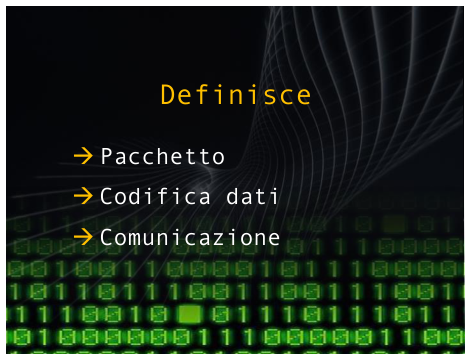
\includegraphics[width=0.50\textwidth,
                    trim=20 100 20 60, % L B R T
                    clip]
                    {images/Lez05_p03_fig_05}
  % \caption{Sommario}
  % \label{fig:Lez15_p06_fig_02}
\end{figure}
\FloatBarrier
\noindent


SOAP definisce un pacchetto in cui definisce il messaggio e come poter manipolare, elaborare il messaggio trasportato, come i dati sono codificati e la comunicazione, quindi la procedura per la richiesta e la fornitura delle risposte.

\FloatBarrier
\begin{figure}[H]
  \centering
  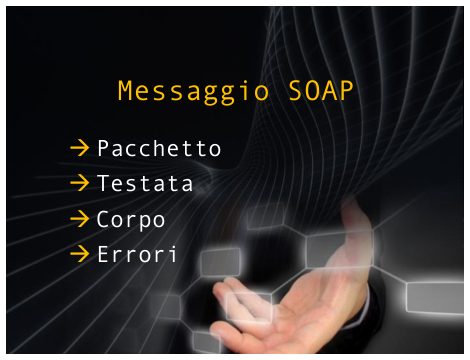
\includegraphics[width=0.50\textwidth,
                    trim=20 80 20 60, % L B R T
                    clip]
                    {images/Lez05_p03_fig_06}
  % \caption{Sommario}
  % \label{fig:Lez15_p06_fig_02}
\end{figure}
\FloatBarrier
\noindent


Un messaggio SOAP è costituito da un pacchetto che identifica il documento XML come messaggio SOAP, una testata, un header, come descrittore, come contenitore di metainformazione per l'istradamento, la sicurezza e la gestione delle transazioni o dell'orchestrazione dei servizi.

Il corpo che contiene sia le chiamate, sia le risposte o meglio informazioni che riguardano le richieste di servizio, le invocazioni di servizio e le ricerche di disponibilità di un servizio.
Inoltre il messaggio trasporta anche la descrizione degli errori eventualmente occorsi durante le operazioni di ricerca o comunque di comunicazione durante l'attività dei servizi, di erogazione dei servizi.

\FloatBarrier
\begin{figure}[H]
  \centering
  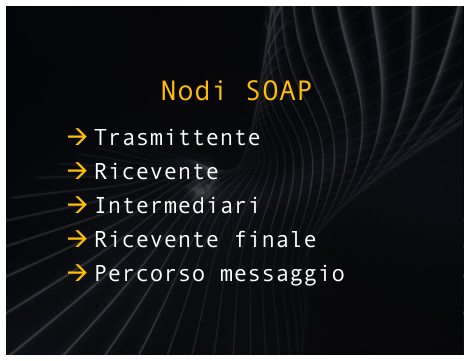
\includegraphics[width=0.50\textwidth,
                    trim=20 60 20 60, % L B R T
                    clip]
                    {images/Lez05_p04_fig_01}
  % \caption{Sommario}
  % \label{fig:Lez15_p06_fig_02}
\end{figure}
\FloatBarrier
\noindent

Un elemento fondamentale per il simple object access protocol sono i nodi.
Bene sono diversi tipi, il nodo trasmittente è il nodo da cui parte la richiesta.
Il ricevente è il destinatario di un messaggio che può essere però intermediario, cioè un nodo che riceve un messaggio per inoltrarlo a sua volta fino a raggiungere il ricevente finale, cioè il nodo che riceve la richiesta dell'utente, può soddisfarla e elabora il messaggio SOAP a questo scopo.

Infine il percorso del messaggio che è la sequenza di tutti i nodi che hanno letto e inoltrato o elaborato il messaggio.
Vediamo che questo paradigma, questo protocollo che sostiene il paradigma architetturale per la gestione dei servizi, deve fornire una definizione delle specifiche per la realizzazione di applicazioni che sono composte con elementi gestiti da attori differenti, attori remoti che offrono dei servizi, che offrono delle applicazioni per il momento sconosciute.

Quello che viene richiesta è la raggiungibilità di queste applicazioni, di questi sostegni ai servizi e quello che viene fornito quindi sono le regole di comportamento, i meccanismi, gli attori, i partecipanti a questo meccanismo o a questo paradigma paradigma architetturale.

\FloatBarrier
\begin{figure}[H]
  \centering
  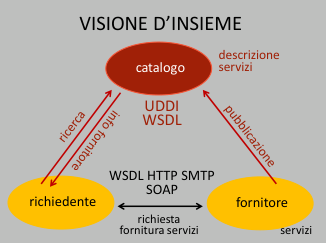
\includegraphics[width=0.50\textwidth,
                    trim=00 00 00 00, % L B R T
                    clip]
                    {images/Lez05_p04_fig_02}
  % \caption{Sommario}
  % \label{fig:Lez15_p06_fig_02}
\end{figure}
\FloatBarrier
\noindent

Ma vediamo un attimo una sintesi grafica, vediamo l'architettura di una visione di insieme, che ci mostri una visione di insieme del funzionamento dei servizi web.
Abbiamo i tre attori, il catalogo archivio dei servizi web, i servizi sono descritti in web service description language, il catalogo è alimentato da qui e indichiamo ovviamente un solo fornitore di servizi, ma è un indicativo di una classe di sviluppatori, qualunque sviluppatore di un servizio utile lo pubblica al catalogo descritto nell'opportuno linguaggio.
Il richiedente, cioè un'applicazione o un utente che avesse bisogno di un'attività, prima di realizzare un'opportuna applicazione può effettuare una ricerca attraverso i cataloghi di web services inviando una richiesta secondo il protocollo UDDI, se la richiesta può essere soddisfatta dal catalogo, quindi se viene recuperato un servizio che svolga attività compatibili o rilevanti per quelle richieste, ecco che il catalogo invia le informazioni per raggiungere il fornitore, l'erogatore, quindi le indicazioni sulla macchina da accedere, il server erogatore del servizio e informazioni sull'interfaccia, quindi sul modo di accedere a questi servizi.

I protocolli che vengono usati in questo scambio e fornitura di servizi sono, come avevamo già visto, Simple Object Access Protocol, il WSDL, quindi i servizi sono descritti, sono proposti in questo linguaggio e per la trasmissione sono utilizzati anche i protocolli utilizzati per la navigazione, i protocolli ipertestuale e il Simple Mail Transfer Protocol per l'invio di pacchetti di dati formattati come mail.

\FloatBarrier
\begin{figure}[H]
  \centering
  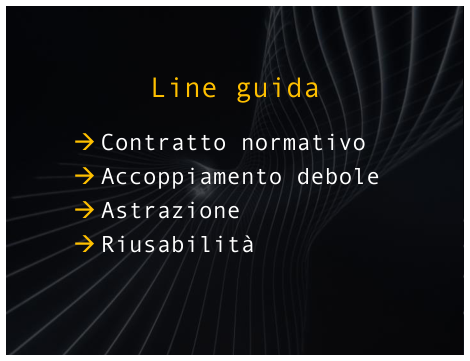
\includegraphics[width=0.50\textwidth,
                    trim=60 80 60 60, % L B R T
                    clip]
                    {images/Lez05_p04_fig_03}
  % \caption{Sommario}
  % \label{fig:Lez15_p06_fig_02}
\end{figure}
\FloatBarrier
\noindent

Vediamo ora che questo protocollo ha necessità di un contratto normativo, delle linee guida.

La prima indica il contratto normativo che permette di svincolare il funzionamento, la progettazione, di un servizio complesso dall'erogazione di servizi dalla loro implementazione.

In seguito viene richiesto come linea guida che i singoli servizi abbiano un accoppiamento debole, significa che siano svincolati funzionalmente dagli altri servizi.

Poi l'astrazione, quindi diano una descrizione non di dettaglio delle attività e la loro possibile riusabilità.

Vediamo per quanto riguarda questo insieme di linee guida che poi completeremo che l'uso di servizi web permette o implica a questo punto avendo un contratto normativo potremmo parlare di imporre la separazione dalla descrizione del funzionamento all'implementazione.
Un contratto normativo presenta le regole di richiesta e di fornitura dei servizi in maniera svincolata dal loro funzionamento.

Stiamo parlando di applicativi che possono essere implementati da qualsiasi possibile fornitore in qualsiasi tipo di linguaggio di programmazione, in qualsiasi modo di programmazione, pur che rispetti determinate caratteristiche, determinati protocolli per la propria pubblicazione e l'interfacciamento con gli altri servizi.

\FloatBarrier
\begin{figure}[H]
  \centering
  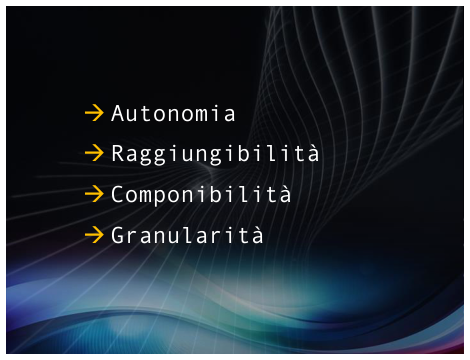
\includegraphics[width=0.50\textwidth,
                    trim=60 80 60 60, % L B R T
                    clip]
                    {images/Lez05_p04_fig_04}
  % \caption{Sommario}
  % \label{fig:Lez15_p06_fig_02}
\end{figure}
\FloatBarrier
\noindent

Proseguiamo con le linee guida.
I servizi devono essere autonomi, indipendenti dagli altri servizi, se non essere a conoscenza degli eventuali servizi che possano essere composti con questi per il completamento del servizio complesso.

La raggiungibilità.
I cataloghi sono proprio lo strumento per la raggiungibilità.
I servizi sono componibili e di una granularità opportuna.

Stiamo con questo pacchetto di quattro linee guida, riferendoci alla possibilità di utilizzare applicativi sconosciuti prima dell'accesso, prima delle informazioni, delle descrizioni che ci sono fornite dal catalogo.

Quindi questi servizi dovranno poter essere riutilizzati, composti con altri che noi sceglieremo da altri fornitori, va da sé che l'autonomia di questi singoli componenti di strutture complesse che andranno orchestrate debbano essere autonomi.
Quindi ogni servizio verrà erogato con un'applicazione a sé stante che fornisce tutti i dati necessari alla propria esecuzione.

\FloatBarrier
\begin{figure}[H]
  \centering
  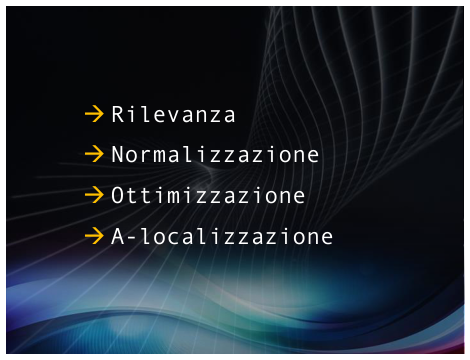
\includegraphics[width=0.50\textwidth,
                    trim=60 80 60 60, % L B R T
                    clip]
                    {images/Lez05_p04_fig_05}
  % \caption{Sommario}
  % \label{fig:Lez15_p06_fig_02}
\end{figure}
\FloatBarrier
\noindent

Vediamo ora l'ultimo gruppo.
La rilevanza.
Un web service deve svolgere delle attività interessanti, normalizzate per minimare la ridondanza, ottimizzate nella loro esecuzione e a-localizzate.
A priori non si sa dove è localizzato, qual è il fornitore che lo eroga.

Stiamo qui focalizzandoci sulla granularità dei servizi, quindi da una parte dimensione dell'attività, ampiezza dell'attività svolta da un singolo servizio, dall'altra parte sul fatto che questa attività deve avere un interesse, deve essere possibile, deve svolgere un'attività logicamente consistente e deve poter essere richiesto da qualsiasi parte.

Qui l'intervento, come abbiamo visto, dei cataloghi che permettono proprio la ricerca di queste attività che possano essere rilevanti, quindi svolgano delle funzioni logiche consistenti ma minimali, senza però indicare la locazione in rete.

\FloatBarrier
\begin{figure}[H]
  \centering
  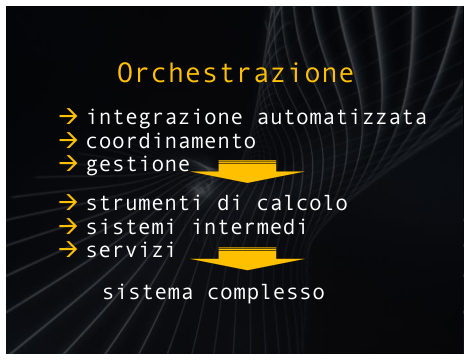
\includegraphics[width=0.50\textwidth,
                    trim=40 20 20 40, % L B R T
                    clip]
                    {images/Lez05_p04_fig_06}
  % \caption{Sommario}
  % \label{fig:Lez15_p06_fig_02}
\end{figure}
\FloatBarrier
\noindent

Per poter organizzare questi web service interviene l'orchestrazione.
L'orchestrazione permette l'integrazione automatizzata, il coordinamento di questi servizi e la gestione.

Queste tre attività sono svolti su strumenti di calcolo, sistemi di erogazione di servizi intermedi e minimalmente sui servizi, allo scopo di costituire un sistema complesso.

L'orchestrazione permette di scindere l'organizzazione di un sistema complesso basato sui web services dalla loro implementazione.
Abbiamo visto che il paradigma di riferimento non impone vincoli implementativi, non impone la locazione degli elementi di software, non impone neanche il tipo di organizzazione.
L'orchestrazione allora non è altro che un modo, uno strumento, per poter descrivere il comportamento che devono avere nel loro funzionamento i vari elementi costituenti, i vari granuli, si parla di granularità dei servizi, dei vari elementi costituenti, un'organizzazione basata su una regia comune.
Ai servizi viene data la modalità di interagire uno con l'altro e come comunicare, come richiamarsi, come invocare la complementarità del successivo servizio.

\FloatBarrier
\begin{figure}[H]
  \centering
  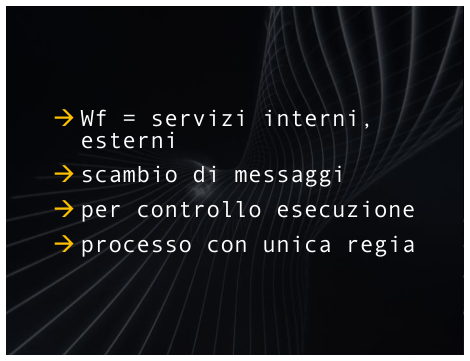
\includegraphics[width=0.50\textwidth,
                    trim=40 80 20 80, % L B R T
                    clip]
                    {images/Lez05_p05_fig_01}
  % \caption{Sommario}
  % \label{fig:Lez15_p06_fig_02}
\end{figure}
\FloatBarrier
\noindent

L'orchestrazione fa riferimento anche a workflow, per servizi interni e servizi esterni, allo scambio di messaggi sia per il controllo dell'esecuzione sia per il controllo della regia che è unica.

Abbiamo visto allora che a completamento l'orchestrazione ha come riferimento la regia contenuta o descritta, presentata dal workflow.

Per il richiamo dei servizi interni intendiamo quelli prodotti dal richiedente, quelli utilizzabili in locali, richiamabili direttamente, ma anche quelli esterni che vanno ricercati.

Lo scambio di messaggi nell'orchestrazione è l'unico modo per poter coordinare l'attività dei vari elementi autonomi, sia nel controllo della loro esecuzione, quindi il completamento della loro attività e la correttezza della loro attività, sia per lo svolgimento con un'unica regia.
Il workflow definisce le modalità, la sequenza o il tipo di parallelismo di concorrenzialità che devono avere i servizi per essere orchestrati correttamente, cioè per concorrere alla realizzazione del servizio complessivo.
Quindi stiamo definendo non la struttura, il progetto di dettaglio di un sistema complesso, ma stiamo definendo il protocollo di comportamento, il protocollo di esecuzione e di interattività dei singoli elementi costituenti.

\FloatBarrier
\begin{figure}[H]
  \centering
  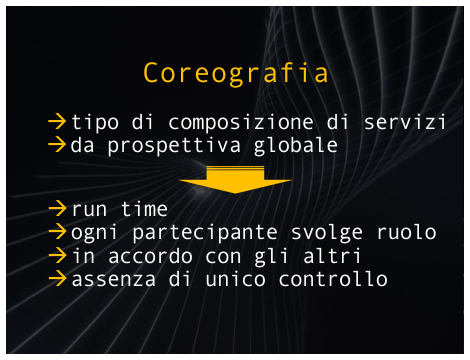
\includegraphics[width=0.50\textwidth,
                    trim=40 40 10 40, % L B R T
                    clip]
                    {images/Lez05_p05_fig_02}
  % \caption{Sommario}
  % \label{fig:Lez15_p06_fig_02}
\end{figure}
\FloatBarrier
\noindent

L'orchestrazione ha una regia, i servizi che vengono coordinati in maniera orchestrata, quindi i servizi che vengono orchestrati seguono un workflow, seguono una unica regia, ma abbiamo un altro modo di definire il modo di comportamento di un servizio complesso ed è la coreografia, che è un altro tipo di composizione dei servizi visti da una prospettiva globale, però vengono definiti i comportamenti in esecuzione.

Ogni partecipante si limita a svolgere un ruolo in accordo con gli altri, vi è l'assenza di un unico controllo.
Ecco che ora stiamo proponendo un coordinamento del tutto differente dall'orchestrazione.
Anche il controllo della attività, oltre che la sua esecuzione, è distribuita nei vari servizi.
Quindi questo è un esempio, un caso estremo di progettazione dei servizi o di attualizzazione di un'architettura service oriented.

I singoli servizi, i singoli elementi costituenti il servizio complesso vengono utilizzati attribuendo a ognuno o realizzandoli ognuno con le proprie informazioni necessarie, i propri strumenti di calcolo, ma anche in questo caso le regole per la composizione con gli altri servizi.

Durante l'esecuzione ogni elemento, ogni servizio, avrà gli strumenti, avrà le capacità per coordinarsi con gli altri elementi secondo il progetto definito dalla coreografia.
Ma la coreografia, abbiamo visto, definisce regole di interazione tra i vari o specifiche di interazione tra i vari elementi, ma evita una strategia comune.

In conclusione, proporrei uno spunto di riflessione.
Prima dello spunto di riflessione vi esorto però a ripercorrere il percorso dal paradigma, il percorso mentale, dal paradigma di architettura, quindi il modello di definizione, agli elementi, alle richieste di elementi necessari per la sua attualizzazione.

Quindi quali sono i vari protocolli, quali sono le varie funzionalità, quali sono gli elementi attori fino ai metodi per l'organizzazione, il coordinamento di questo tipo di applicazione, quindi coreografia o unica regia, quindi orchestrazione.

Dopodiché, spunto di riflessione, vi propongo di ideare un servizio riferito al vostro ambito lavorativo o formativo offerto da un fornitore remoto.
Vi sto chiedendo di ideare un'attività rilevante, di interesse quindi per la vostra realtà lavorativa o formativa che sia erogata come servizio mediante un'applicazione sviluppata come web service da qualche fornitore di cui non conoscete l'esistenza.
Quindi effettuare la ricerca di questa possibile attività attraverso il paradigma SOA che abbiamo visto realizzato attraverso i web services.